Aquest capítol presenta l'anàlisi de les dades de seguiment ocular---fixacions i regressions---i la seva relació amb les anotacions del \textit{gold standard} provinents del corpus MuSeD i les explicacions dels models de llenguatge. També analitza les decisions dels participants durant l'experiment.

\section{Anotacions dels participants}

Primer examinem les anotacions binàries de sexisme i les comparem amb el \textit{gold standard}.
Com es mostra a la \autoref{tab:participant_accuracy}, vuit dels deu participants obtenen resultats significativament superiors als esperables per atzar.
Dos participants (F2 i F4) no arriben a la significació estadística, tot i que la seva exactitud (62,5\%) és superior a l'atzar.
Aquests resultats indiquen que, en conjunt, els participants han resolt la tasca amb prou atenció.

Identifiquem els participants amb els codis M1--M5 (homes) i F1--F5 (dones).
M3 i F5 havien estat anotadors de MuSeD i són els participants amb les exactituds més altes.

\iftables
\begin{table}[htbp]
\small
\centering
\begin{tabular}{lcc}
\toprule
\textbf{Participant} & \textbf{Exactitud} & \textbf{valor $p$} \\
\midrule
M3 & 100,0\% & $< 0,001$ ** \\
F5 &  92,5\% & $< 0,001$ ** \\
M1 &  90,0\% & $< 0,001$ ** \\
M5 &  87,5\% & $< 0,001$ ** \\
F1 &  85,0\% & $< 0,001$ ** \\
M2 &  82,5\% & $< 0,001$ ** \\
F3 &  82,5\% & $< 0,001$ ** \\
M4 &  82,5\% & $< 0,001$ ** \\
F2 &  62,5\% & $= 0,077$ ns \\
F4 &  62,5\% & $= 0,077$ ns \\
\bottomrule
\end{tabular}
\caption{Exactitud de cada participant comparada amb l'atzar (prova binomial, bilateral).}
\label{tab:participant_accuracy}
\end{table}
\fi

\subsection{Diferències per gènere}

\iftables
\begin{table}[htbp]
\small
\centering
\begin{tabular}{lll}
\toprule
\textbf{Prova} & \textbf{Estadístic} & \textbf{valor $p$} \\
\midrule
U de Mann-Whitney (exactitud per text) & $U = 1001,5$ & $0,035$ * \\
Exacta de Fisher (errors en texts sexistes) & OR $= 0,72$ & $0,468$ \hphantom{$*$} ns \\
\bottomrule
\end{tabular}
\caption{Comparacions de l'exactitud basades en el gènere del participant. OR=Oportunitat relativa.}
\label{tab:gender}
\end{table}
\fi

%La mitjana d'exactitud és del 82,7\%, la majoria dels participants identifiquen correctament el contingut sexista.
%Això dona validesa a les dades de seguiment ocular recollides.


La \autoref{tab:gender} presenta les comparacions basades en el gènere dels participants.
La prova U de Mann--Whitney sobre l'exactitud per text mostra una diferència significativa, però de petita magnitud.
No obstant això, aquesta diferència no es manté quan examinem específicament els errors en texts sexistes amb la prova exacta de Fisher.

\subsection{Confiança i dificultat de text}

La confiança autoinformada dels participants (escala 1--3) està significativament calibrada amb l'exactitud: una confiança més alta s'associa amb una exactitud més gran ($\rho = 0,29$, $p < 0,001$).
Malgrat la moderada correlació, la tendència és clara i significativa.
De les 400 anotacions, la majoria es fan amb confiança alta: 268 amb confiança 3 (67,0\%), 86 amb confiança 2 (21,5\%) i 46 amb confiança 1 (11,5\%).
L'exactitud augmenta amb el nivell de confiança: 57\% (nivell~1), 74\% (nivell~2) i 90\% (nivell~3).
És a dir, només el 10\% de les anotacions amb confiança alta (27) són incorrectes.

La dificultat dels texts és heterogènia.
Els més difícils, és a dir, els que presenten menys acord amb el \textit{gold standard}, són:

\begin{itemize}
    \item Text 37: 50\% acord (5/10 participants) -- no sexista amb ironia i humor
    \item Text 144: 50\% acord -- sexista amb estereotips i desigualtat
    \item Text 5: 60\% acord -- sexista amb ironia i discriminació
    \item Text 30: 60\% acord -- sexista amb humor i discriminació
    \item Text 107: 60\% acord -- sexista amb desigualtat
\end{itemize}

Aquests texts són bons candidats per a una anàlisi més detallada, ja que podrien representar casos límit o ambigus.
Dels 10 texts amb 100\% d'acord, 5 són sexistes i 5 no.
Els sexistes presenten majoritàriament categories explícites: \textit{estereotips} (3 texts), \textit{desigualtat} (2) i \textit{discriminació} (1).
Això suggereix que el sexisme explícit, basat en \textit{estereotips} o \textit{desigualtat}, és fàcilment identificable pels lectors.
En canvi, cap dels texts amb \textit{ironia} o \textit{humor} apareix en aquest grup de màxima facilitat, fet que confirma que aquestes formes de sexisme subtil són més difícils de detectar.

\subsection{Detecció per subcategories de sexisme}

La \autoref{tab:error_analysis} mostra la taxa d'error individual en la detecció de cadascuna de les subcategories de sexisme definides en el \textit{gold standard}.
L'\textit{humor} presenta la taxa d'error més alta, del 30\%, seguida de \textit{discriminació} (23\%) i \textit{desigualtat} (23\%).
El text~5, classificat com a sexista amb \textit{ironia} i \textit{discriminació}, n'és un exemple il·lustratiu: es tracta d'un diàleg sobre identitat de gènere on l'ús d'ironia (\textit{``Soy un hombre lesbiana''}) fa que la meitat dels participants el classifiquin com a no sexista.

\iftables
\begin{table}[htbp]
\small
\centering
\begin{tabular}{lcc}
\toprule
\textbf{Subcategoria} & \textbf{Errònies / Total} & \textbf{Taxa d'error} \\
\midrule
humor              & 6/20 & 30\% \\
discriminació      & 14/60 & 23\% \\
desigualtat        & 16/70 & 23\% \\
ironia             & 4/20 & 20\% \\
sexisme implícit   & 3/20 & 15\% \\
estereotips        & 16/110 & 15\% \\
\bottomrule
\end{tabular}
\caption{Taxa d'error individual en la detecció de texts sexistes per subcategoria. Cada anotació d'un participant sobre un text sexista és un cas independent: s'agrupen les anotacions errònies (el participant va classificar el text com a no sexista) per subcategoria del \textit{gold standard}.}
\label{tab:error_analysis}
\end{table}
\fi

Per examinar si aquestes diferències són estadísticament significatives, vam fer proves exactes de Fisher per comparar les taxes d'error entre totes les parelles de categories, amb correcció de Bonferroni.
Cap comparació per parelles va resultar significativa, ni abans ni després de la correcció.
Per tant, les diferències observades entre subcategories, per exemple entre \textit{humor} i \textit{estereotips}, podrien deure's a l'atzar.

\section{Record estimulat}

Les entrevistes de \textit{stimulated recall} revelen tres aspectes.
En primer lloc, l'ambigüitat és freqüent: els participants sovint no saben si un text és sexista, especialment quan conté ironia, humor o opinions que es poden interpretar de diverses maneres.
En segon lloc, busquen pistes contextuals per resoldre aquesta ambigüitat. Per exemple, intenten identificar qui parla, quina és la seva posició ideològica o si el text descriu un fet o expressa una opinió.
Finalment, els participants amb experiència prèvia amb el corpus---els anotadors de MuSeD---i els participants amb poc contacte amb el castellà mostren processos de lectura diferents: els primers reconeixen els casos i els processen més ràpidament, mentre que els segons necessiten més relectures.

Aquests resultats confirmen que la detecció de sexisme en texts és una tasca subjectiva, especialment en casos d'ironia o sexisme implícit. També justifiquen l'ús de mètriques de distribució, en lloc de comparacions binàries.
A continuació presentem les observacions més rellevants de les entrevistes, agrupades per text.

\paragraph{Text 4.}
La majoria dels participants identifiquen el text com a sexista, però les estratègies de lectura varien.
Alguns expressen desconfiança inicial (\textit{``ha dubtat, canviaria segons qui ho digui''}) abans de decidir.
Una participant que coneixia el corpus reconeix el cas i expressa ràbia davant l'equiparació entre pedofília i orientació sexual.
En canvi, una altra no sap si l'interlocutor és a favor o en contra, i no es fixa en res en concret.

\paragraph{Text 30.}
Alguns participants contextualitzen ràpidament el text: \textit{``ja s'espera que dirà un comentari sexista''}.
D'altres no ho tenen clar o l'interpreten com a no sexista.
Una participant es fixa en ``ahora'', que interpreta com un possible canvi de punt de vista, i rellegeix el text perquè no sap si descriu un fet sexista o si el text és sexista en si mateix.

\paragraph{Text 37.}
Aquest text, marcat com a no sexista pel \textit{gold standard}, genera opinions dispars.
Alguns l'interpreten com a sexista perquè no diferencia entre sexe i gènere; d'altres, com una caricatura o com un atac al gènere masculí. També hi ha participants que es fixen en la ideologia del forense.

\paragraph{Text 107.}
Els participants es divideixen entre les opcions sexista i no sexista.
Alguns decideixen que és sexista al final, mentre que d'altres el veuen com una simple opinió.
Diversos participants no saben si parla una dona sarcàsticament o un home que fa un acudit sexista.

\paragraph{Text 166.}
Alguns el veuen com una opinió no sexista, mentre que d'altres l'interpreten com un atac al gènere masculí.
Una participant es fixa en ``eres un hombre malo'' com a posicionament de la persona i li sembla discurs d'extrema dreta.

\paragraph{Text 375.}
La majoria entenen que podria ser una crítica, però el \textit{``makes no sense. Gracias''} del final ho fa explícit.
Una participant es fixa en ``feminisme'' i ``todo ofende'', interpretant que primer presenta una situació i després dona la seva opinió.

\paragraph{Text 399.}
Alguns pensen inicialment que es tracta d'un cas sexista, però interpreten el missatge sencer com una crítica.
Una participant es fixa en els sinònims (\textit{``nena, abuelita, doña''}) que reafirmen la posició.


\section{Distribucions d'atenció: comparació amb les anotacions de segments}

%\subsection{Mètriques de distribució ocular}

D'acord amb la justificació del marc teòric, en les comparacions següents prenem la TFD com a mètrica principal d'eye-tracking. La FFD i la FC s'hi incorporen posteriorment com a mesures complementàries de robustesa.

Per a cada parell (participant, text), calculem quatre mètriques que comparen la distribució d'atenció del participant amb les anotacions del \textit{gold standard}. La distribució d'atenció es basa en la TFD normalitzada per token, que expliquem a l'\autoref{app:tfd}; les comparacions amb FFD i FC es presenten a l'apartat~\ref{sec:kl_ikhwantri}.

\begin{itemize}
    \item \textbf{Correlació de Spearman:} mesura la concordança monòtona entre dues distribucions.
    \item \textbf{Entropia creuada (\textit{cross-entropy}, CE):} mesura la divergència probabilística.
    \item \textbf{Divergència de Kullback--Leibler (KL):} mesura la divergència informacional de la TFD respecte de l'anotació.
    \item \textbf{Divergència de Jensen--Shannon (JS):} versió simètrica de la KL, més interpretable.
\end{itemize}
La correlació de Spearman varia entre $-1$ i $1$ (més alta = millor alineament). 
La CE té com a mínim l'entropia de la distribució de referència. 
La divergència KL és positiva i la JS és simètrica i està acotada a $[0, 1]$.
La CE i les dues divergències indiquen millor alineament com menor és el valor.

En 10 dels texts seleccionats, o bé tots els tokens estan anotats com a segments o bé no n'hi ha cap.
Per tant, aquests texts no s'inclouen en aquesta anàlisi, perquè no contenen un senyal discriminant.
La \autoref{tab:per_participant_metrics} mostra els resultats per participant.

\iftables
\begin{table}[htbp]
\small
\centering
\begin{tabular}{lcccc}
\toprule
\textbf{Participant} & \textbf{Spearman} & \textbf{CE} & \textbf{KL} & \textbf{JS} \\
\midrule
F5 & $0,07 \pm 0,20$ & $9,47 \pm 2,33$ & $5,32 \pm 2,33$ & $0,22 \pm 0,07$ \\
F1 & $0,06 \pm 0,19$ & $9,65 \pm 2,12$ & $5,50 \pm 2,12$ & $0,24 \pm 0,07$ \\
M5 & $0,05 \pm 0,16$ & $9,30 \pm 2,03$ & $5,15 \pm 2,03$ & $0,21 \pm 0,07$ \\
F2 & $0,04 \pm 0,21$ & $9,54 \pm 2,17$ & $5,39 \pm 2,17$ & $0,22 \pm 0,07$ \\
M2 & $0,03 \pm 0,13$ & $9,91 \pm 1,86$ & $5,76 \pm 1,86$ & $0,26 \pm 0,06$ \\
F4 & $0,02 \pm 0,17$ & $9,57 \pm 1,76$ & $5,42 \pm 1,76$ & $0,23 \pm 0,06$ \\
M1 & $0,02 \pm 0,18$ & $9,55 \pm 1,84$ & $5,40 \pm 1,84$ & $0,23 \pm 0,06$ \\
M3 & $0,02 \pm 0,17$ & $10,08 \pm 2,19$ & $5,93 \pm 2,19$ & $0,28 \pm 0,07$ \\
M4 & $0,02 \pm 0,15$ & $10,12 \pm 2,13$ & $5,97 \pm 2,13$ & $0,29 \pm 0,07$ \\
F3 & $0,01 \pm 0,10$ & $10,07 \pm 2,06$ & $5,92 \pm 2,06$ & $0,28 \pm 0,07$ \\
\bottomrule
\end{tabular}
\caption{Mètriques de distribució per participant (mitjana $\pm$ desviació estàndard).}
\label{tab:per_participant_metrics}
\end{table}
\fi

Les correlacions de Spearman són properes a zero per a tots els participants, cosa que indica una concordança gairebé nul·la entre la distribució d'atenció i les anotacions de segments.
La divergència JS mitjana és 0,25 (en una escala de 0 = distribucions idèntiques a 1 = totalment diferents), fet que indica una separació moderada: no tan baixa com la que s'observa entre lectors i anotadors (0,12), però molt lluny de la divergència total (0,78--0,84) que es troba entre els models i els segments.
% TODO: mirar figura
% La \autoref{fig:exemple_visual} mostra un exemple representatiu d'aquesta distribució per al text~30, on les zones d'alt TFD coincideixen amb les zones anotades com a sexistes.
% \begin{figure}[htbp]
% \centering
% \includegraphics[width=0.95\textwidth]{../src/pdfs_examples/example_30.pdf}
% \caption{Exemple visual de la distribució d'atenció (TFD) i prominència del model per al text~30. Les barres superiors representen la prominència de cada mètode (Saliency, Input$\times$Gradient, IG, LRP) i les barres inferiors mostren l'atenció humana (TFD). El color vermell indica tokens dins de segments anotats com a sexistes.}
% \label{fig:exemple_visual}
% \end{figure}

\subsection{Alineament per categories de sexisme}

Analitzem l'alineament entre l'atenció humana i les anotacions de segments de dues maneres complementàries.
Primer examinem les mètriques de distribució dins dels segments anotats amb cada tipus d'etiqueta.
La \autoref{tab:per_label_metrics} presenta els resultats.
Les correlacions de Spearman són baixes per a totes les etiquetes, però les divergències varien.
La \textit{desigualtat ideològica} presenta la JS més alta (0,50), mentre que \textit{estereotips} (0,23) i \textit{objectificació} (0,24) presenten les més baixes.
Categories implícites com \textit{sexisme implícit}, \textit{humor} i \textit{ironia} mostren un alineament relativament bo, superior al de categories explícites com \textit{desigualtat/discriminació}, \textit{sexisme reportat} o \textit{desigualtat ideològica}.

\iftables
\begin{table}[htbp]
\small
\centering
\begin{tabular}{lcccc}
\toprule
\textbf{Etiqueta} & \textbf{Spearman} & \textbf{CE} & \textbf{KL} & \textbf{JS} \\
\midrule
desig. ideol.           & $0,06 \pm 0,13$ & $9,20$ & $5,98$ & $0,50$ \\
desigualtat/discrim.    & $0,06 \pm 0,15$ & $9,80$ & $5,99$ & $0,37$ \\
crítica                 & $0,04 \pm 0,17$ & $10,00$ & $5,90$ & $0,29$ \\
sexisme reportat        & $0,01 \pm 0,11$ & $10,42$ & $6,27$ & $0,40$ \\
estereotips             & $0,04 \pm 0,14$ & $9,40$ & $5,25$ & $0,23$ \\
sexisme implícit        & $0,06 \pm 0,16$ & $9,60$ & $5,45$ & $0,25$ \\
objectificació          & $0,06 \pm 0,14$ & $9,50$ & $5,35$ & $0,24$ \\
ironia                  & $0,03 \pm 0,16$ & $9,80$ & $5,65$ & $0,28$ \\
humor                   & $0,05 \pm 0,19$ & $9,70$ & $5,55$ & $0,26$ \\
\bottomrule
\end{tabular}
\caption{Mètriques de distribució per tipus d'etiqueta del segment (mitjana creuada entre participants i texts).}
\label{tab:per_label_metrics}
\end{table}
\fi

A continuació, a la \autoref{tab:binary_js}, separem els texts segons la presència o absència de cada categoria binària del \textit{gold standard} i calculem la divergència JS.
La presència de \textit{desigualtat} augmenta la JS de 0,24 a 0,33, cosa que indica dificultats especials.
\textit{Humor} i \textit{ironia} mostren patrons inversos: quan són presents, la JS disminueix fins a 0,21, mentre que augmenta fins a 0,26 quan són absents. \textit{Objectificació} i \textit{sexisme reportat} també presenten divergències més altes quan són presents.

\iftables
\begin{table}[htbp]
\small
\centering
\begin{tabular}{lcc}
\toprule
\textbf{Categoria} & \textbf{JS (negatiu)} & \textbf{JS (positiu)} \\
\midrule
sexista          & 0,24 & 0,27 \\
ironia           & 0,26 & 0,21 \\
humor            & 0,26 & 0,21 \\
sexisme implícit & 0,26 & 0,20 \\
estereotips      & 0,25 & 0,26 \\
desig. ideol.    & 0,24 & 0,33 \\
discriminació    & 0,25 & 0,25 \\
objectificació   & 0,26 & 0,32 \\
crítica          & 0,27 & 0,23 \\
sexisme reportat & 0,26 & 0,32 \\
\bottomrule
\end{tabular}
\caption{Divergència JS entre els segments anotats i TFD per categoria binària. Negatiu = categoria absent; Positiu = categoria present.}
\label{tab:binary_js}
\end{table}
\fi


\section{Anàlisi de regressions oculars}

% \subsection{Resum general de regressions}

En el conjunt de parells participant--text, detectem un total de 8.642 regressions, amb una mitjana de $216 \pm 77$ regressions per text.
La majoria són regressions dins de la mateixa línia (\textit{within-line}), que representen el 89,8\%; les regressions entre línies (\textit{between-line}) constitueixen el 10,2\% restant.
En l'anàlisi seguim la convenció de \textcite{rayner2009eye}: el token de destí és aquell cap al qual es dirigeix la regressió (on torna el lector per reprocessar), i el token d'origen és aquell des del qual es produeix (on s'interromp la lectura per tornar enrere). Vegeu l'\autoref{app:tfd} per a la definició completa.

\subsection{\textit{Baselines} individuals per participant}

\iftables
\begin{table}[htbp]
\small
\centering
\begin{tabular}{lccr}
\toprule
\textbf{Participant} & \textbf{Taxa de regressió (\%)} & \textbf{Mitjana FD (ms)} & \textbf{$n$ regressions} \\
\midrule
F1 & 25 & 226 & 1,395 \\
F5 & 21 & 267 & 1.283 \\
M1 & 21 & 232 & 1.145 \\
M4 & 20 & 252 & 908 \\
F4 & 22 & 244 & 781 \\
M5 & 17 & 264 & 685 \\
M2 & 19 & 237 & 625 \\
F3 & 15 & 268 & 613 \\
F2 & 22 & 199 & 597 \\
M3 & 15 & 244 & 495 \\
\bottomrule
\end{tabular}
\caption{Baselines de regressió per participant. Taxa de regressió = proporció de fixacions que són regressions. Mitjana FD = durada mitjana de fixació.}
\label{tab:participant_baselines}
\end{table}
\fi
La \autoref{tab:participant_baselines} presenta la línia de base de regressió de cada participant, incloses la taxa de regressió i la durada mitjana de fixació.
La durada mitjana de fixació global és 248,8 ms.
Les diferències individuals són notables.
La taxa de regressió varia entre el 15\% i el 25\%, valors lleugerament més elevats que la taxa típica del 10--15\% en lectors competents en anglès~\cite{conklinEyeTrackingGuideApplied2018}.
Aquesta variabilitat és compatible amb les diferències individuals en les estratègies de lectura, com ara la tendència a revisar segments anteriors per resoldre ambigüitats o confirmar la comprensió.

\subsection{Tokens significatius}

Calculem la puntuació z (unitat tipificada) per a cada token, comparant el nombre de regressions amb la línia de base del participant.
Després d'aplicar la correcció de Benjamini--Hochberg\footnote{Controla la taxa de descobriment fals ajustant els p-valors per limitar la proporció esperada de falsos positius entre tots els resultats significatius.}, identifiquem 2.797 tokens de destí i 2.795 tokens d'origen significatius.
És a dir, són tokens als quals els participants tornen significativament més sovint del que esperaríem per atzar.

Per validar els resultats de la puntuació z, fem 10.000 permutacions per a cada parell (participant, text), mantenint l'estructura de les dades.
Amb la correcció de la taxa de falsos descobriments de Benjamini--Hochberg, obtenim 84 tokens de destí i 94 tokens d'origen significatius.
La concordança entre els dos mètodes és moderada:

\begin{itemize}
    \item \textbf{Destí:} 53 tokens significatius per ambdós mètodes, 2.744 només per la \textit{z-score}, 31 només per permutació
    \item \textbf{Origen:} 84 tokens significatius per ambdós mètodes, 2.711 només per la \textit{z-score}, 10 només per permutació
\end{itemize}

La puntuació z identifica més tokens significatius que la permutació perquè assumeix independència entre observacions, mentre que la permutació té en compte l'estructura de les dades.

\subsection{Punts focals de regressió lèxics}

Entre tots els tokens significatius identificats, el 52,8\% són paraules buides (preposicions, conjuncions, etc.), que filtrem amb la biblioteca NLTK\footnote{https://www.nltk.org/}.
Per a cadascun dels 40 texts, seleccionem els 10 tokens significatius amb la puntuació z més alta i prioritzem els que també són significatius per permutació ($q < 0,05$).
%Quan no hi havia prou tokens significatius per permutació, es completaven amb tokens significatius només per \textit{z-score}.
Anomenem aquests tokens \textit{punts focals}. 
La \autoref{tab:top_hotspots} presenta els 40 punts focals lèxics més significatius---un per text---ordenats per puntuació z.
\iftables
\begin{table}[htbp]
%\small
%\footnotesize
\centering
\begin{tabular}{clclc}
\toprule
\textbf{Text} & \textbf{Destí} & $z$ & \textbf{Origen} & $z$ \\
\midrule
4 & llegado & $6,64$ & progresismo & $5,16$ \\
5 & lesbiana & $7,11$ & mientras & $6,88$ \\
23 & sexual & $6,47$ & Sígueme & $6,79$ \\
30 & forense & $5,75$ & Feministas & $4,91$ \\
37 & sobrevibir & $2,94$ & Imaginate & $3,41$ \\
45 & patriarcal & $5,37$ & explicar & $5,89$ \\
55 & ahorita & $8,14$ & solo & $8,00$ \\
59 & miren & $4,64$ & saben & $4,34$ \\
60 & la & $3,80$ & no & $4,65$ \\
62 & existe & $5,67$ & hombre & $5,74$ \\
76 & creen & $7,93$ & Administrativa & $8,00$ \\
78 & Infojobs & $6,11$ & mercado & $5,95$ \\
99 & anticuado & $6,25$ & jerárquicas & $6,61$ \\
106 & mujer & $5,64$ & cumplidos & $5,08$ \\
107 & aquí & $4,42$ & ley & $5,17$ \\
124 & nací & $6,87$ & pena & $6,95$ \\
133 & real & $6,42$ & antecedentes & $6,11$ \\
136 & culturales & $6,66$ & cualidades & $6,46$ \\
143 & ridículo & $8,75$ & habilidad & $8,81$ \\
144 & tóxica & $6,82$ & lado & $6,52$ \\
148 & parejas & $6,43$ & relacionarse & $5,90$ \\
150 & pide & $5,75$ & oír & $5,42$ \\
151 & literalmente & $7,95$ & favor & $8,05$ \\
166 & pueden & $3,25$ & sense & $3,65$ \\
201 & años & $7,00$ & siempre & $6,47$ \\
214 & opinas & $4,64$ & gracias & $4,83$ \\
215 & Pues & $5,63$ & beneficiado & $7,00$ \\
217 & bestia & $5,93$ & lecciones & $6,02$ \\
327 & puedes & $5,84$ & voy & $6,22$ \\
352 & marzo & $5,91$ & abrazo & $5,77$ \\
356 & natural & $6,47$ & civilización & $6,59$ \\
357 & supiese & $6,40$ & cuenta & $6,48$ \\
359 & acceder & $5,43$ & violación & $4,85$ \\
362 & voy & $7,27$ & pasando & $7,36$ \\
364 & idiomas & $6,92$ & respuesta & $6,27$ \\
373 & pasto & $4,49$ & verdad & $5,26$ \\
375 & tema & $6,33$ & problema & $6,14$ \\
383 & seguidor & $5,58$ & largo & $5,32$ \\
390 & patriarcado & $4,17$ & violentas & $4,09$ \\
399 & chamaquito & $5,75$ & doña & $5,43$ \\
\bottomrule
\end{tabular}
\caption{Punts focals de destí i origen per text, sense puntuació. Destí = token on els lectors regressionen més sovint ($z$ més alt en direcció TO); Origen = token des del qual els lectors fan més regressions ($z$ més alt en direcció FROM).}
\label{tab:top_hotspots}
\end{table}
\fi
En destaquem tres aspectes:
\begin{itemize}
    \item \textbf{Paraules relacionades amb el gènere:} termes com ``lesbiana'', ``mujer'', ``patriarcal'', ``tóxica'', ``parejas'', ``mujeres'', ``hombres'', ``jerárquicas'' i ``femenino'' apareixen sovint entre els punts focals, en consonància amb el contingut sexista dels texts. En total, 28 tokens (9,3\%) fan referència directa a conceptes de gènere o a relacions de poder.
    \item \textbf{Distribució morfològica:} l'anàlisi de les categories gramaticals dels 300 tokens que no són paraules buides mostra que els punts focals són majoritàriament substantius (41,1\%), seguits de verbs (21,9\%), adjectius (16,6\%) i adverbis (8,6\%). En el context de gènere, molts adjectius descriuen qualitats o atributs (\textit{lesbiana}, \textit{tóxica}, \textit{patriarcal}, \textit{culturales}, \textit{jerárquicas} i \textit{femenino}). Els verbs sovint expressen accions o judicis (\textit{ahorita}, \textit{odian}, \textit{creen} i \textit{explicar}).
    \item \textbf{Direcció de regressió:} la majoria dels punts focals són tokens de destí, és a dir, tokens als quals els lectors tornen més sovint. Això suggereix que revisen elements temàticament rellevants.
\end{itemize}


\subsection{Relació amb les anotacions de segments}

Per examinar si els tokens amb més atenció ocular corresponen a les zones anotades com a sexistes, comparem els 2.881 tokens significatius segons la puntuació z amb les anotacions de segments del \textit{gold standard}.
Del total, 2,458 tokens significatius (85,3\%) es troben dins d'un interval anotat. Això indica una forta associació entre les zones de més atenció dels lectors i les zones etiquetades com a sexistes.

No obstant això, la prova exacta de Fisher per text no assoleix significació estadística en cap cas, possiblement per manca de potència (mitjana de 4--10 tokens anotats per text i 10 participants). L'efecte global---el 85,3\% dels tokens significatius es troben dins de segments---és molt superior al que esperaríem per atzar.

La \autoref{tab:spearman_coverage} mostra la correlació de Spearman entre la cobertura de cada segment (proporció de tokens anotats) i la taxa de regressió mitjana per text, estratificada per categoria d'etiqueta.
L'única correlació significativa és a la categoria ``sexista'': els texts sexistes presenten taxes de regressió més altes.
Per tant, els lectors semblen fer més regressions davant del contingut sexista, possiblement perquè aquest contingut requereix més reprocessament cognitiu.

\iftables
\begin{table}[htbp]
\small
\centering
\begin{tabular}{lccr}
\toprule
\textbf{Categoria} & \textbf{$\rho$} & \textbf{valor $p$} & \textbf{$n$ texts} \\
\midrule
sexista          & 0,429 & 0,006 * & 20 \\
discriminació   & 0,273 & 0,088 {\hphantom{*}} & 6 \\
crítica         & $-0,233$ & 0,147 {\hphantom{*}} & 19 \\
estereotips     & 0,204 & 0,207 {\hphantom{*}} & 14 \\
sexisme implícit& 0,199 & 0,218 {\hphantom{*}} & 12 \\
humor           & 0,078 & 0,634 {\hphantom{*}} & 6 \\
\bottomrule
\end{tabular}
\caption{Correlació de Spearman entre cobertura de segment (proporció de tokens anotats) i taxa mitjana de regressió per text, estratificat per categoria. $n$ = nombre de texts amb cobertura $> 0$ per a cada categoria.}
\label{tab:spearman_coverage}
\end{table}
 \fi

\subsection{Punts focals dins de segments per tipus d'etiqueta}

A la \autoref{tab:span_hotspots} identifiquem punts focals de regressió significatius dins dels intervals anotats per a cada tipus d'etiqueta. Els ponderem per l'invers de la longitud del segment per evitar un biaix cap als segments llargs.

\iftables
\begin{table}[htbp]
\small
\centering
\begin{tabular}{lcrcr}
\toprule
\textbf{Etiqueta} & \textbf{$n$ punts focals} & \textbf{$z$ mitjà} & \textbf{Clúster mitjà} & \textbf{Long. segment} \\
\midrule
crítica                 & 42 & $5,81$ & 56,0 & 60,4 \\
estereotips             & 30 & $5,98$ & 55,1 & 58,1 \\
desigualtat/discrim.    & 30 & $5,70$ & 50,5 & 53,3 \\
sexisme implícit        & 24 & $5,58$ & 37,7 & 37,7 \\
ironia                  & 16 & $5,13$ & 39,6 & 39,6 \\
humor                   & 18 & $5,21$ & 29,8 & 47,0 \\
desig. ideol.           & 10 & $5,20$ & 17,2 & 28,6 \\
objectificació          & 10 & $5,87$ & 20,4 & 37,8 \\
sexisme reportat        &  8 & $5,86$ & 53,8 & 53,8 \\
\bottomrule
\end{tabular}
\caption{Punts focals de regressió per tipus d'etiqueta de segment, ponderats per $1/\text{longitud}$.}
\label{tab:span_hotspots}
\end{table}
\fi

\textit{Crítica} és l'etiqueta amb més punts focals (42), seguida d'\textit{estereotips} (30) i de les categories \textit{desigualtat} i \textit{discriminació} (30 en conjunt).
Els punts focals amb les puntuacions z més altes il·lustren com els lectors reprocessen regions clau del text:

\ex. \label{ex:hotspot143} \textbf{Text 143, objectificació i estereotips} (origen ``Cómo'', $z = 6{,}65$): el text comença amb ``¿Cómo ser gracioso y conquistar sin hacer el ridículo?'', un consell de seducció. Els lectors interrompen la lectura a l'inici i tornen enrere després de llegir les situacions exemples (la dona dient ``és hora d'anar al llit''), com si necessitessin verificar si la tècnica de malinterpretació intencional és realment el que es descriu. El clúster més petit per a \textit{objectificació} (9 tokens) vs.\ \textit{estereotips} (23 tokens) suggereix que la relectura per identificar l'objectificació és més localitzada, mentre que per als estereotips abasta un radi més ampli.

\ex. \label{ex:hotspot55} \textbf{Text 55, crítica} (destí ``ahorita'', $z = 8{,}14$, clúster de 98 tokens): el text critica el feminisme dient que ``no és res més que odiar als homes''. ``Ahorita'' és un marcador temporal que ancora la crítica al present. Els lectors tornen a rellegir des de punts posteriors fins a aquesta paraula, possiblement per situar temporalment la comparació amb els feminicidis diaris i verificar si la coherència argumentativa es manté.

\ex. \label{ex:hotspot76} \textbf{Text 76, desigualtat/discriminació} (origen ``Administrativa'', $z = 8{,}00$, clúster de 73 tokens): el text planteja àrees de treball (minería, construcció, plataformes petrolíferes) i conclou amb ``Administrativa per nosaltres''. Els lectors regressen des d'aquesta conclusió discriminatòria fins a les preguntes anteriors, reclamant el context complet de la comparació per confirmar que la ironia és efectivament sexista.

\section{Mètriques d'eye-tracking}

A més de les mètriques basades en regressions, analitzem la TFD, la FFD i la FC per token.

\subsection{Mètriques d'eye-tracking per token}

En primer lloc, comparem la TFD, la FFD i la FC mitjanes per text entre els 20 texts sexistes i els 20 no sexistes amb la prova de Mann--Whitney.
\iftables
\begin{table}[htbp]
\small
\centering
\begin{tabular}{lccr}
\toprule
\textbf{Mètode} & \textbf{Sexistes} & \textbf{No sexistes} & \textbf{$p$} \\
\midrule
TFD (\%) & $1,87 \pm 0,52$ & $2,41 \pm 1,33$ & 0,473 \\
FFD (ms) & $198,2 \pm 6,1$ & $201,0 \pm 5,6$ & 0,133 \\
FC       & $1,95 \pm 0,37$  & $2,03 \pm 0,37$  & 0,209 \\
\bottomrule
\end{tabular}
\caption{TFD, FFD i FC mitjanes per text segons etiqueta binària (Mann-Whitney, bilateral).}
\label{tab:ffd_fc_binary}
\end{table}
\fi
La \autoref{tab:ffd_fc_binary} mostra les mètriques mitjanes per text.
Els texts no sexistes tendeixen a presentar valors lleugerament més alts de TFD, FFD i FC, però les diferències són petites i no significatives.

En segon lloc, per avaluar si els tokens dins dels segments anotats com a sexistes reben més atenció, calculem les puntuacions z de TFD, FFD i FC per participant, respecte de la seva mitjana global, i comparem els tokens dins i fora dels segments.
\iftables
\begin{table}[htbp]
\small
\centering
\begin{tabular}{lccr}
\toprule
\textbf{Mètode} & \textbf{Dins segment} & \textbf{Fora segment} & \textbf{$p$} \\
\midrule
TFD z-score & $+0,045$ & $-0,284$ & $< 0,001$ * \\
FFD z-score & $+0,003$ & $-0,018$ & \hphantom{$<$} 0,741 \hphantom{*} \\
FC z-score  & $+0,020$ & $-0,126$ & $< 0,001$ * \\
\bottomrule
\end{tabular}
    \caption{Z-scores de TFD, FFD i FC per tokens dins ($n = 18\,708$) vs.\ fora ($n = 2\,973$) dels segments anotats (Mann-Whitney, bilateral).}
\label{tab:ffd_fc_span}
\end{table}
\fi
La \autoref{tab:ffd_fc_span} mostra diferències significatives per a la TFD i la FC: els tokens dins dels segments anotats com a sexistes reben més fixacions i durant més temps que els tokens fora dels segments.
En canvi, la FFD no presenta diferències significatives.

La \autoref{tab:metrics_correlation} mostra les correlacions de Spearman entre parelles de mètriques.
La TFD i la FC presenten una correlació forta ($\rho = 0,623$), com era esperable, ja que totes dues mesuren l'atenció acumulada i el reprocessament deliberat. En canvi, la FFD captura la reacció inicial, més automàtica.
La correlació entre la TFD i la FFD és moderada ($\rho = 0,318$).
La correlació feblement negativa entre la FFD i la FC ($\rho = -0,070$) suggereix que els tokens que reben la primera fixació més llarga no són necessàriament els que reben més visites.
És possible que els lectors revisitin deliberadament els fragments sexistes, tot i que la primera impressió que els produeixen no sigui diferent de la de la resta del text.
Aquest patró és coherent amb els resultats de l'anàlisi de regressions, en què els tokens dins dels segments presenten taxes de retorn més altes.
\iftables
\begin{table}[htbp]
\small
\centering
\begin{tabular}{lccr}
\toprule
\textbf{Parell} & \textbf{$\rho$ de Spearman} & \textbf{$p$} \\
\midrule
TFD vs.\ FFD & 0,318 & $< 0,001$ * \\
TFD vs.\ FC  & 0,623 & $< 0,001$ * \\
FFD vs.\ FC  & $-0,070$ & $< 0,001$ * \\
\bottomrule
\end{tabular}
\caption{Correlació de Spearman entre les tres mètriques d'eye-tracking per token.}
\label{tab:metrics_correlation}
\end{table}
\fi

\subsection{Prominència dels models vs.\ mètriques d'eye-tracking}

Per extreure la prominència de cada model, fem servir quatre mètodes d'interpretabilitat: N'extraiem la prominència amb quatre mètodes d'interpretabilitat: Saliency, Input$\times$Gradient, Integrated Gradients (IG) i Layer-wise Relevance Propagation (LRP).
La \autoref{tab:model_vs_eye_tracking} presenta la correlació de Spearman entre la prominència de cada token---el valor absolut de l'atribució del model---i les tres mètriques d'eye-tracking (TFD, FFD i FC), promitjades entre participants per als 40 texts.
\iftables
\begin{table}[htbp]
\small
\centering
\begin{tabular}{lcccc}
\toprule
\textbf{Model} & \textbf{Mètode} & \textbf{$\rho$ TFD} & \textbf{$\rho$ FFD} & \textbf{$\rho$ FC} \\
\midrule
BETO & IG & 0,068 & $-0,036$ & 0,113 \\
BETO & Input$\times$Gradient & 0,068 & $-0,038$ & 0,116 \\
BETO & LRP & 0,070 & $-0,044$ & 0,115 \\
BETO & Saliency & 0,075 & $-0,042$ & 0,122 \\
MrBERT-es & IG & 0,037 & $-0,062$ & 0,083 \\
MrBERT-es & Input$\times$Gradient & 0,045 & $-0,057$ & 0,088 \\
MrBERT-es & LRP & 0,041 & $-0,051$ & 0,081 \\
MrBERT-es & Saliency & 0,049 & $-0,054$ & 0,092 \\
mBERT & IG & 0,070 & $-0,039$ & 0,116 \\
mBERT & Input$\times$Gradient & 0,068 & $-0,040$ & 0,114 \\
mBERT & LRP & 0,081 & $-0,045$ & 0,127 \\
mBERT & Saliency & 0,076 & $-0,042$ & 0,124 \\
\bottomrule
\end{tabular}
\caption{Correlació de Spearman: prominència del model vs.\ mètriques d'eye-tracking (mitjana sobre 40 texts).}
\label{tab:model_vs_eye_tracking}
\end{table}
\fi
Les correlacions són positives, però febles per a la TFD i la FC.
Per tant, els tokens als quals els models assignen més importància coincideixen parcialment amb els que reben més atenció dels lectors.
La FFD mostra una correlació lleugerament negativa, coherent amb el fet que la primera fixació no discrimina entre zones sexistes i no sexistes, com ja hem observat.

mBERT obté les correlacions més altes ($\rho = 0,076$ per a la TFD i $\rho = 0,124$ per a la FC amb Saliency), seguit de BETO ($\rho = 0,075$ i $0,122$) i MrBERT-es ($\rho = 0,049$ i $0,092$).
En mBERT, LRP mostra correlacions similars o lleugerament superiors a les de Saliency ($\rho = 0,081$ per a la FC); en la resta de models, els resultats són comparables.

\section{Comparació entre atenció humana i prominència de models}

En aquesta secció comparem tres models preentrenats (mBERT, BETO i MrBERT-es) amb dues referències: les anotacions de segments del \textit{gold standard} i l'atenció humana mesurada amb eye-tracking.
N'extraiem la prominència amb Saliency, Input$\times$Gradient, IG i LRP.

Totes les comparacions de distribucions utilitzen filtratge de paraules buides (vegeu l'ablació a l'Apèndix~\ref{sec:stopword_ablation}).

\subsection{Prominència del model vs.\ anotacions de segments}

En primer lloc, comparem les distribucions de prominència dels models amb les anotacions de segments sexistes del corpus MuSeD.

\subsubsection{Solapament}

Avaluem fins a quin punt les paraules amb més prominència coincideixen amb les paraules incloses en els segments anotats com a sexistes pel \textit{gold standard}.
La \autoref{tab:model_vs_spans} mostra la superposició per a cinc llindars: l'1\%, el 3\%, el 5\%, el 10\% i el 20\% dels tokens amb més prominència.
\iftables
\begin{table}[htbp]
\small
\centering
\begin{tabular}{lcccccc}
\toprule
\textbf{Model} & \textbf{Mètode} & \textbf{1\%} & \textbf{3\%} & \textbf{5\%} & \textbf{10\%} & \textbf{20\%} \\
\midrule
BETO & IG & 0,907 & 0,904 & 0,888 & 0,888 & 0,904 \\
BETO & Input$\times$Gradient & 0,890 & 0,887 & 0,871 & 0,871 & 0,887 \\
BETO & LRP & 0,890 & 0,887 & 0,871 & 0,871 & 0,887 \\
BETO & Saliency & 0,890 & 0,887 & 0,871 & 0,871 & 0,887 \\
MrBERT-es & IG & \textbf{0,922} & \textbf{0,918} & \textbf{0,918} & \textbf{0,918} & \textbf{0,918} \\
MrBERT-es & Input$\times$Gradient & 0,890 & 0,887 & 0,887 & 0,887 & 0,887 \\
MrBERT-es & LRP & 0,890 & 0,887 & 0,887 & 0,887 & 0,887 \\
MrBERT-es & Saliency & 0,890 & 0,887 & 0,887 & 0,887 & 0,887 \\
mBERT & IG & 0,919 & 0,916 & 0,900 & 0,900 & 0,916 \\
mBERT & Input$\times$Gradient & 0,890 & 0,887 & 0,871 & 0,871 & 0,887 \\
mBERT & LRP & 0,890 & 0,887 & 0,871 & 0,871 & 0,887 \\
mBERT & Saliency & 0,890 & 0,887 & 0,871 & 0,871 & 0,887 \\
\bottomrule
\end{tabular}
\caption{Solapament: paraules amb prominència més alta vs.\ paraules dins dels segments anotats, per a diferents llindars de selecció.}
\label{tab:model_vs_spans}
\end{table}
\fi
La superposició és alta independentment del llindar (87,1\%--92,2\%), tot i que disminueix lleugerament al 5\%--10\% respecte de l'1\%--3\%.
Aquest patró suggereix que els tokens amb prominència més extrema---l'1\%--3\% superior---es troben gairebé sempre dins dels segments. Quan ampliem el llindar al 5\%--10\%, hi incorporem alguns tokens externs; al 20\%, la proporció torna a augmentar perquè els nous tokens interns compensen aquesta incorporació.
El mètode IG produeix una superposició consistentment superior a la de Saliency, Input$\times$Gradient i LRP.
Això indica que les atribucions d'IG estan més concentrades en les paraules clau dels segments.

\subsubsection{Distribucions de prominència}

La \autoref{tab:model_vs_span_dist} compara les distribucions de prominència dels models amb les anotacions de segments.

\iftables
\begin{table}[htbp]
\small
\centering
\begin{tabular}{lcccc}
\toprule
\textbf{Model} & \textbf{Mètode} & \textbf{CE} & \textbf{KL} & \textbf{JS} \\
\midrule
BETO & IG & 24,45 & 21,15 & 0,781 \\
BETO & Input$\times$Gradient & 24,55 & 21,26 & 0,795 \\
BETO & LRP & 24,71 & 21,43 & 0,790 \\
BETO & Saliency & 24,51 & 21,22 & 0,776 \\
MrBERT-es & IG & 25,56 & 22,32 & 0,830 \\
MrBERT-es & Input$\times$Gradient & 25,69 & 22,40 & 0,837 \\
MrBERT-es & LRP & 25,67 & 22,36 & 0,833 \\
MrBERT-es & Saliency & 25,67 & 22,38 & 0,827 \\
mBERT & IG & 24,39 & 21,10 & 0,779 \\
mBERT & Input$\times$Gradient & 24,54 & 21,26 & 0,791 \\
mBERT & LRP & 24,56 & 21,27 & 0,786 \\
mBERT & Saliency & 24,51 & 21,22 & 0,775 \\
\bottomrule
\end{tabular}
\caption{Mètriques de distribució: prominència del model vs.\ anotacions de segment, amb paraules buides filtrades (mitjana sobre 40 texts).}
\label{tab:model_vs_span_dist}
\end{table}
\fi

Una JS mitjana d'aproximadament 0,78--0,84 indica una divergència substancial, però no total, entre la distribució de prominència dels models i les anotacions de segments.
Aquesta divergència és esperable: els segments marquen només una part del text com a sexista, mentre que la prominència es distribueix entre tots els tokens.
Les diferències entre mètodes d'interpretabilitat són petites, cosa que suggereix que la distribució de prominència és similar independentment del mètode utilitzat.

\subsubsection{Alineament per tipologia d'etiqueta}

La \autoref{tab:model_typology} desglossa l'alineament entre la prominència dels models i l'atenció humana per tipus d'etiqueta de segment.
Les xifres són una mitjana sobre les 12 combinacions de model i mètode.
La variabilitat entre combinacions és moderada: el rang de JS dins de cada model entre mètodes varia de 0,16 (MrBERT-es) a 0,27 (BETO), i el rang entre models dins de cada mètode varia de 0,19 (Input$\times$Gradient) a 0,28 (LRP).
La combinació que produeix la JS més baixa és BETO amb LRP (0,789), i la més alta és MrBERT-es amb IG (0,866), cosa que indica que l'elecció del model té més pes que la del mètode.

\iftables
\begin{table}[htbp]
\small
\centering
\begin{tabular}{lccccc}
\toprule
\textbf{Etiqueta} & \textbf{Prom. (dins)} & \textbf{Prom. (fora)} & \textbf{$\rho$ TFD} & \textbf{$\rho$ FC} & \textbf{JS} \\
\midrule
crítica                 & 0,036 & 0,000 & 0,042 & 0,097 & 0,741 \\
estereotips             & 0,028 & 0,027 & 0,096 & 0,131 & 0,850 \\
sexisme reportat        & 0,009 & 0,019 & $-0,036$ & $-0,012$ & 0,887 \\
desigualtat/discrim.    & 0,017 & 0,029 & 0,089 & 0,160 & 0,798 \\
humor                   & 0,042 & 0,000 & 0,092 & 0,183 & 0,836 \\
ironia                  & 0,022 & 0,019 & 0,129 & 0,259 & 0,822 \\
sexisme implícit        & 0,039 & 0,030 & 0,150 & 0,325 & 0,871 \\
objectificació          & 0,007 & 0,027 & 0,138 & 0,198 & 0,895 \\
desig. ideol.           & 0,035 & 0,027 & --- & --- & 0,818 \\
\bottomrule
\end{tabular}
\caption{Mètriques per tipus d'etiqueta del segment: prominència del model dins de cada tipologia (mitjana sobre texts, models i mètodes).}
\label{tab:model_typology}
\end{table}
\fi

Les principals observacions són les següents. \textit{Crítica} i \textit{humor} concentren la prominència dins del segment i no en presenten fora, cosa que suggereix que els models identifiquen clarament aquestes categories.
En canvi, \textit{sexisme reportat} i \textit{objectificació} presenten menys prominència dins del segment que fora, fet que apunta a dificultats per identificar-les.
El text~144 (\textit{``mujer tóxica''}) n'és un cas representatiu: malgrat estar anotat com a sexista amb \textit{estereotips} i \textit{desigualtat}, els models no concentren la prominència en el segment, cosa que confirma la dificultat de detectar estereotips sense marcadors explícits de discriminació.

Pel que fa a les correlacions amb les mètriques d'eye-tracking, \textit{sexisme implícit} mostra els valors més alts amb FC i TFD. Això indica que els models i els lectors coincideixen més en aquesta tipologia subtil.
\textit{Ironia} també presenta correlacions relativament altes, compatibles amb una captura similar del fenomen.
Finalment, la JS més baixa correspon a \textit{crítica}, que mostra la concordança més alta entre les distribucions dins i fora del segment.

\newpage
\subsection{Prominència del model vs.\ TFD}

En segon lloc, la \autoref{tab:model_vs_human_dist} compara les distribucions de prominència dels models amb l'atenció humana (TFD).
La JS entre els models i la TFD (0,77--0,84) és pràcticament la mateixa que entre els models i els segments (0,78--0,84).
Les diferències entre mètodes són igualment petites.
\iftables
\begin{table}[htbp]
\small
\centering
\begin{tabular}{lcccc}
\toprule
\textbf{Model} & \textbf{Mètode} & \textbf{CE} & \textbf{KL} & \textbf{JS} \\
\midrule
BETO & IG & 24,43 & 21,15 & 0,778 \\
BETO & Input$\times$Gradient & 24,51 & 21,21 & 0,790 \\
BETO & LRP & 24,62 & 21,31 & 0,782 \\
BETO & Saliency & 24,47 & 21,17 & 0,770 \\
MrBERT-es & IG & 25,54 & 22,34 & 0,825 \\
MrBERT-es & Input$\times$Gradient & 25,68 & 22,38 & 0,835 \\
MrBERT-es & LRP & 25,73 & 22,41 & 0,835 \\
MrBERT-es & Saliency & 25,66 & 22,37 & 0,825 \\
mBERT & IG & 24,35 & 21,09 & 0,777 \\
mBERT & Input$\times$Gradient & 24,51 & 21,21 & 0,787 \\
mBERT & LRP & 24,55 & 21,25 & 0,782 \\
mBERT & Saliency & 24,47 & 21,17 & 0,770 \\
\bottomrule
\end{tabular}
\caption{Mètriques de distribució: prominència del model vs.\ atenció humana (TFD), amb paraules buides filtrades (mitjana sobre 40 texts).}
\label{tab:model_vs_human_dist}
\end{table}
\fi

\subsection{Resum de les tres comparacions}\label{sec:resum_tripartit}

La \autoref{tab:tripartite_summary} resumeix les tres comparacions: models--segments, models--TFD i TFD--segments.
La divergència JS més baixa és la que s'observa entre la TFD i les anotacions de segments.
Llavors, anotadors i lectors comparteixen una visió similar de sexisme.
La divergència més alta és la que es dona entre els models i les anotacions de segments, cosa que indica que els models de llenguatge distribueixen la prominència de manera substancialment diferent de les persones.
\iftables
\begin{table}[htbp]
\small
\centering
\begin{tabular}{lccc}
\toprule
\textbf{Parell} & \textbf{JS (Saliency)} & \textbf{JS (IG)} & \textbf{JS (LRP)} \\
\midrule
Model -- Segments  & 0,78--0,83 & 0,78--0,83 & 0,79--0,83 \\
Model -- TFD        & 0,77--0,83 & 0,78--0,83 & 0,78--0,84 \\
TFD -- Segments     & 0,12 (ref.) & --- & --- \\
\bottomrule
\end{tabular}
\caption{Resum de divergència JS per als tres parells de distribucions, amb paraules buides filtrades. La TFD vs.\ segments prové de l'ablació~\ref{tab:stopword_ablation} (JS mitjana = 0,12).}
\label{tab:tripartite_summary}
\end{table}
\fi

\subsection{Precisió del model i divergència KL respecte a l'atenció humana}\label{sec:kl_ikhwantri}

Per comprovar si l'alineament amb l'atenció humana es relaciona amb el rendiment de classificació, seguim la proposta de \textcite{soodInterpretingAttentionModels2020}.
Per a cada combinació de model i mètode, calculem la correlació entre la divergència KL respecte de la TFD i la precisió per text.
La \autoref{tab:sood_metric} recull aquestes correlacions.
\iftables
\begin{table}[htbp]
\small
\centering
\begin{tabular}{llrrrr}
\toprule
\textbf{Model} & \textbf{Mètode} & \textbf{Precisió (\%)} & \textbf{$\rho$ TFD} & \textbf{$\rho$ FFD} & \textbf{$\rho$ FC} \\
\midrule
BETO & IG & 61,1 & $+0,236$ & $+0,159$ & $+0,208$ \\
BETO & Input$\times$Gradient & 62,2 & $+0,125$ & $+0,042$ & $+0,104$ \\
BETO & LRP & 62,2 & $+0,308$ & $+0,230$ & $+0,287$ \\
BETO & Saliency & 62,2 & $+0,193$ & $+0,078$ & $+0,172$ \\
MrBERT-es & IG & 74,2 & $+0,190$ & $+0,107$ & $+0,223$ \\
MrBERT-es & Input$\times$Gradient & 75,7 & $+0,088$ & $+0,024$ & $+0,083$ \\
MrBERT-es & LRP & 75,7 & $+0,024$ & $+0,035$ & $-0,012$ \\
MrBERT-es & Saliency & 75,7 & $+0,083$ & $+0,053$ & $+0,077$ \\
mBERT & IG & 57,6 & $-0,193$ & $-0,174$ & $-0,206$ \\
mBERT & Input$\times$Gradient & 54,1 & $-0,234$ & $-0,203$ & $-0,234$ \\
mBERT & LRP & 54,1 & $-0,249$ & $-0,249$ & $-0,254$ \\
mBERT & Saliency & 54,1 & $-0,259$ & $-0,213$ & $-0,244$ \\
\bottomrule
\end{tabular}
\caption{Correlació de Spearman entre divergència KL (model vs.\ TFD) i rendiment del model per text. Cap correlació és estadísticament significativa.}
\label{tab:sood_metric}
\end{table}
\fi

\begin{figure}[!ht]
\centering
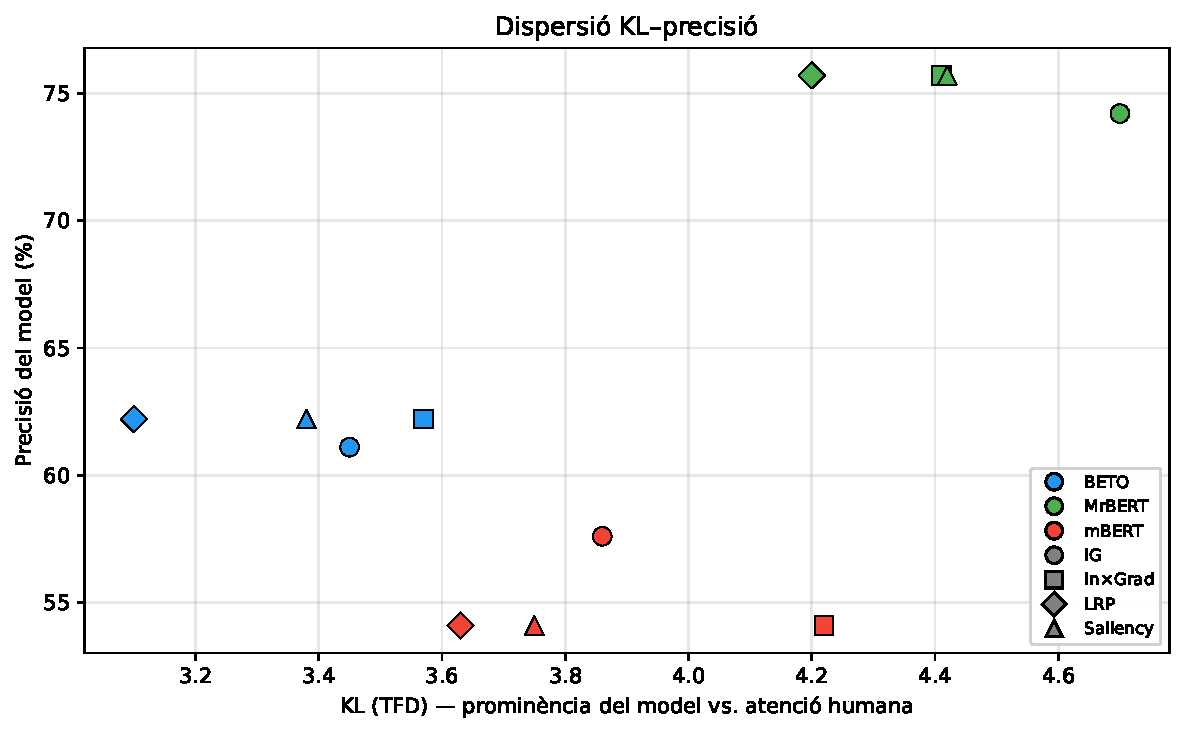
\includegraphics[width=\textwidth]{figures/sd_performance_curve.pdf}
\caption{Dispersió KL--precisió: cada punt representa una combinació de model i mètode d'interpretabilitat. Els colors indiquen els models i les formes, els mètodes.}
\label{fig:sd_performance}
\end{figure}
La \autoref{tab:sood_metric} i la \autoref{fig:sd_performance} mostren la mateixa conclusió des de dues perspectives.
Cap correlació és estadísticament significativa. BETO i MrBERT-es presenten correlacions generalment positives, mentre que mBERT presenta correlacions negatives; tanmateix, la variabilitat entre mètodes no permet establir una relació sistemàtica.
La figura fa explícita aquesta dissociació: MrBERT-es combina una precisió més alta amb valors de KL més grans, mentre que BETO mostra el patró contrari.
Per tant, la similitud amb l'atenció humana i el rendiment de classificació semblen mesurar propietats diferents, en línia amb \textcite{ikhwantriLookingDeepEyes2023}.

Per comprovar que aquesta conclusió no depèn de la mètrica ocular escollida, comparem la divergència KL obtinguda amb TFD, FFD i FC, seguint la proposta d'\textcite{ikhwantriLookingDeepEyes2023}.
La \autoref{tab:ikhwantri_sd} presenta aquesta anàlisi de robustesa.
\iftables
\begin{table}[!ht]
\small
\centering
\begin{tabular}{llrrr}
\toprule
\textbf{Model} & \textbf{Mètode} & \textbf{KL (TFD)} & \textbf{KL (FFD)} & \textbf{KL (FC)} \\
\midrule
BETO & IG & 3,45 & 3,52 & 3,34 \\
BETO & Input$\times$Gradient & 3,57 & 3,64 & 3,46 \\
BETO & LRP & 3,10 & 3,21 & 2,99 \\
BETO & Saliency & 3,38 & 3,48 & 3,27 \\
MrBERT-es & IG & 4,70 & 4,77 & 4,59 \\
MrBERT-es & Input$\times$Gradient & 4,41 & 4,55 & 4,31 \\
MrBERT-es & LRP & 4,20 & 4,30 & 4,12 \\
MrBERT-es & Saliency & 4,42 & 4,54 & 4,33 \\
mBERT & IG & 3,86 & 3,91 & 3,76 \\
mBERT & Input$\times$Gradient & 4,22 & 4,27 & 4,12 \\
mBERT & LRP & 3,63 & 3,75 & 3,53 \\
mBERT & Saliency & 3,75 & 3,86 & 3,65 \\
\bottomrule
\end{tabular}
\caption{Divergència KL per model, mètode i mètrica ocular. Valors més baixos indiquen major similitud entre la distribució de prominència del model i l'atenció humana.}
\label{tab:ikhwantri_sd}
\end{table}
\fi

La FC produeix valors lleugerament més baixos i la FFD, més alts en totes les combinacions, mentre que la TFD queda en una posició intermèdia.
Tanmateix, no triem la TFD només perquè minimitzi la KL, sinó també perquè acumula la durada de totes les fixacions i és, per tant, la mètrica més comparable amb una distribució de prominència acumulada.
